\documentclass{article}

\usepackage[widepage]{repsty}
\usepackage{subcaption}

\newcommand{\W}{\Omega}
\newcommand{\w}{\omega}
\newcommand{\MDM}{{}^\mathrm{MDM}}
\newcommand{\EDM}{{}^\mathrm{EDM}}
\newcommand{\CW}{{}^\mathrm{CW}}
\newcommand{\CCW}{{}^\mathrm{CCW}}



\begin{document}
\title{Frequency domain method for the dEDM search}
We will start by briefly describing the two presently known approaches to measuring the deuteron EDM in a storage ring:
\begin{itemize}
\item the BNL Frozen Spin method;
\item Ivan Koop's Spin Wheel.
\end{itemize}

\section{Known methodologies}
According to the T-BMT equation~\eqref{eq:TBMT}, the storage ring method for measuring the deuteron EDM of necessity induces a radial $\vec\W\EDM$ and a vertical $\vec\W\MDM$ frequency, due to the guiding B-filed. Since the frequencies are orthogonal, they add up in squares, so that the particle spin precesses about a near-vertical axis (because the radial EDM contribution is much smaller than the vertical MDM), with a frequency $\w  = \sqrt{\w_{MDM}^2 + \w_{EDM}^2}$. In such a configuration, $\w_{EDM}$ is drowned by the much higher $\w_{MDM}$.

This problem can be solved by reducing the MDM precession to zero, i.e., fulfilling the Frozen Spin (FS) condition.

\begin{equation}\label{eq:TBMT}
  \begin{cases}
    \vec\W\MDM &= -\alpha_0\bkt*{\alpha_1\vec B + \alpha_2\vec\beta\times\vec E}, \\
    \vec\W\EDM &= -\alpha_0\eta\bkt*{\vec E + \vec\beta\times\vec B}.
  \end{cases}
\end{equation}

For protons, whose anomalous magnetic moment is positive, the beam energy can be adjusted so that the FS condition is fulfilled. Since there does not exist such a ``magic'' energy for the deuteron, in the original BNL proposal a radial electric field was added such that $\vec\W\MDM = \vec 0$ (in the rest frame), and the growth of the vertical polarization component $\Delta P_V$ over a prolonged period of time was measured.~\cite{BNL_proposal}

The immediate challenge one faces with the vanilla FS approach is the EDM effect size. At the sensitivity limit of the experiment, the polarization rotation angle is about one microradian, a problematic figure for polarimetry. The EDM effect size problem itself can be addressed via the Spin Wheel (SW) method.~\cite{Mane:SpinWheel}

The core idea of the SW method consists in adding a controlled MDM rotation about the radial axis, by means of a transverse magnetic dipole, in order to get a measurable signal. Then, by varying the MDM contribution of the combined signal, the EDM component, whose action remains unchanged during the dipole field sweep, can be extracted.

\section{Element misalignment}
As noted in~\cite[p. 24]{BNL_proposal}, electric and magnetic field imperfections cause a first-order systematic error in the $\w\EDM$ estimate. Element misalignment is the primary cause of field imperfections.

Assuming a realistic value of 100 microns installation error, simulations show that the fields generated induce an MDM precession at about 50--100 rad/sec.~\cite{Senichev:FDM} This, of course, completely invalidates the original BNL FS method, because instead of observing a slow, EDM-driven vertical polarization growth, one gets a sinusoidal signal oscillating at 8--16 Hz. Neither does the SW modification provide any way of disentangling the EDM precession from the misalignment-generated MDM precession.

%% The geometric phase error is due to the non-commutativity of spin rotations. It happens when the spin rotation axis deviates from one of the coordinate system axes, i.e., the rotation occurs in three dimensions. This means that unless one can reduce the misalignments to the degree where the radial EDM component of rotation completely dominates all others, it is actually beneficial to go the SW way and maximize the radial MDM rotation (see Figure~\ref{fig:GeomPhase}).

%% \begin{figure}
%%   \centering
%%   \begin{subfigure}[b]{.5\textwidth}\centering
%%     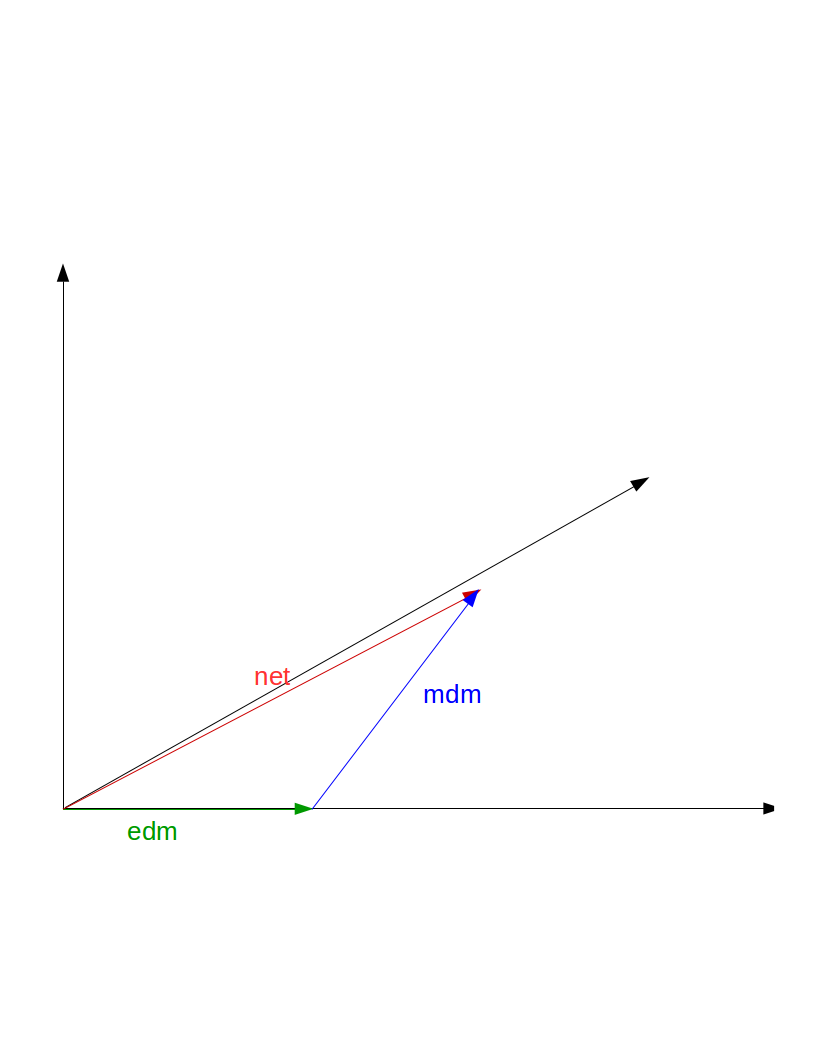
\includegraphics[width=\textwidth]{img/geometric_phase_1}
%%     \caption{Spin rotation axis with reduced element misalignments. The deviation from either of the coordinate system axes is large, and so is geometric phase error.}
%%   \end{subfigure}~
%%   \begin{subfigure}[b]{.5\textwidth}\centering
%%     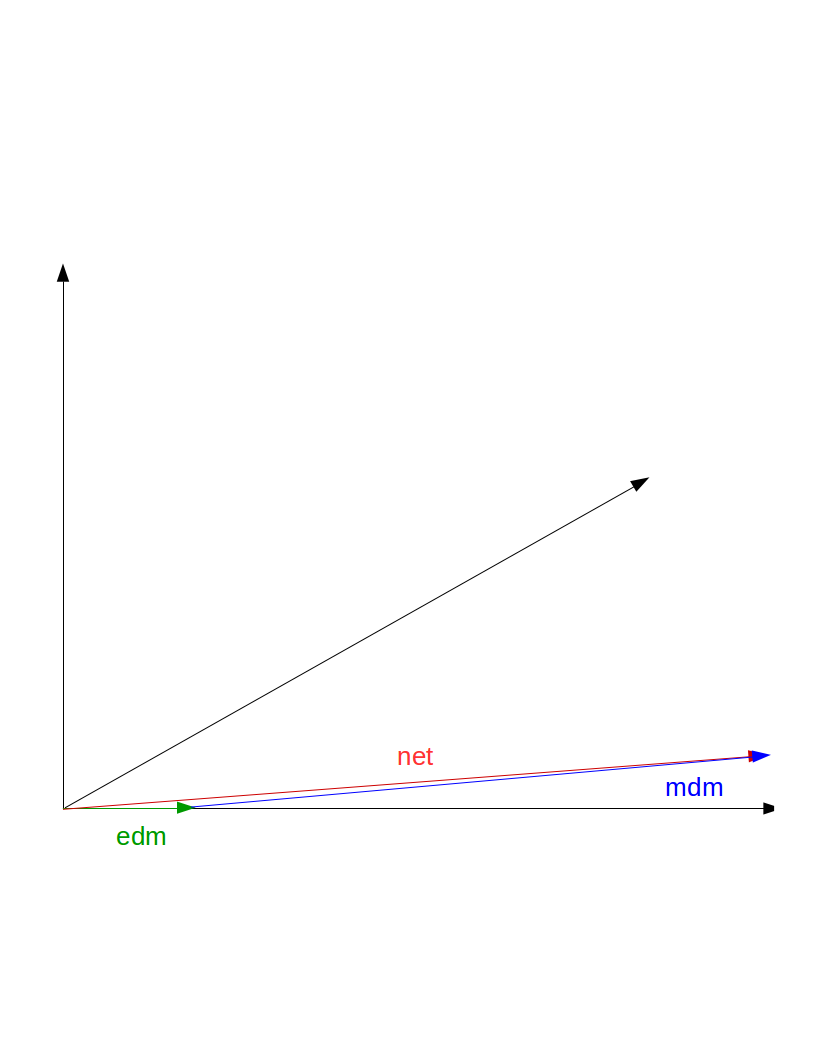
\includegraphics[width=\textwidth]{img/geometric_phase_2}
%%     \caption{Spin rotation axis with an emphasized radial MDM precession; the error is greatly diminished.}
%%   \end{subfigure}
%% \caption{Geometric phase error source.\label{fig:GeomPhase}}
%% \end{figure}

\section{The Frequency Domain methodology}
In view of the misalignment problem described above, it is obvious that a successful methodology will require measurement of a precession frequency. Hence the name: ``Frequency Domain.'' Since a combined EDM + MDM precession is being observed, the next step is to separate the EDM and MDM components. This can be achieved by injecting the beam in opposite directions, and adding up the results. Since both $\vec B$, and $\vec\beta$ change sign, while $\vec E$ remains constant, going from CW to CCW:
\begin{align}
  \w_x\CW &= \w_x\CW\MDM + \w_x\EDM, \\
  \w_x\CCW &= -\w_x\CCW\MDM + \w_x\EDM, \\
  \shortintertext{and so}
  \hat\w_x\EDM &= \frac12\bkt{\w_x\CW + \w_x\CCW} + \frac12\bkt{\w_x\CW\MDM - \w_x\CCW\MDM}.
\end{align}

The several aspects of concern are:
\begin{enumerate}
\item The necessity of a double injection for the computation of a single statistic. The problem here is that we cannot guarantee that the two beams follow the same orbit, and hence experience the same fields. This is problematic for two reasons: \label{itm:Injection}
  \begin{inparaenum}[a)]
  \item a spin rotation is proportional to the experienced field strength, and
  \item spin rotations are not commutative.
  \end{inparaenum}
  
  \item The necessity of reversing the polarity of the guiding field. This is essentially the same problem (due to a different cause) as above: the reversed magnetic field must have the same absolute value as the direct one, else $\W\MDM$ is not reproduced. \label{itm:Polarity}
\end{enumerate}

Below we argue that double injection does not pose a problem, so long as 
\begin{inparaenum}[a)]
\item the frozen spin condition is strictly observed (rotations only occur in one plane), and
\item the parameter $\gamma_{eff}(\gamma_s, x_0, y_0, \sfrac{\Delta p_0}{p_s})$ is kept constant.
\end{inparaenum}
We will also provide a methodology for ensuring that the MDM precession frequency in the y-z plane is reproduced with sufficient precision.

\section{Effective gamma}
Consider the injection space $(x,y,d)$, where $x$, $y$, are the initial offsets of the particle from the reference orbit, and $d := \frac{\Delta\gamma}{\gamma_0}$ is the energy deviation. A particle injected into the storage ring can then be represented by a point in injection space. Each point in the injection space corresponds to an orbit traveled by the particle. We introduce the concept of gamma effective as an equivalence relation on injection space: if two points in injection space are characterized by the same spin tune, they are said to possess the same gamma effective.

The origin of the notion can be traced to decoherence studies in the storage ring for the dEDM experiment,~\cite{Senichev:StorageRingMethod} where it is instrumental in understanding the mechanism by which sextupole fields can be used in order to increse the spin coherence time. Here, we will sketch an outline of the arguments presented in~\cite{Senichev:StorageRingMethod} and~\cite{Senichev:Decoh}.

We start with the expressions for the spin tune in the E-,B-fields:
\begin{equation}\label{eq:spin_tune}
  \begin{cases}
    \nu^B(\gamma) = \gamma B,\\
    \nu^E(\gamma) = \bkt{\frac{1}{\gamma^2-1}-G}\gamma\beta^2.
  \end{cases}
\end{equation}

A particle off the reference orbit is involved in two types of oscillations: betatron and synchrotron, and so describes a 6D ellipsoid in phase space. Its projection on the $(z, \Delta\gamma)$ plane is an ellipse, offset from the energy level $\gamma_s$ of the synchronous particle, and described by:~\cite[p. 2580]{Senichev:Decoh}
\begin{equation}\label{eq:delta_gamma}
  \Delta\gamma(t) = \Delta\gamma_m\cos\Omega_s t - \frac{\beta^2}{\eta}\bkt*{\bkt{\alpha_1 - \frac{\eta}{\gamma_s^2}}\frac{\Delta\gamma_m^2}{\beta_s^2} + \gamma^2\bkt{\frac{\Delta L}{L}}_\beta},
\end{equation}
where $\frac{\Delta L}{L}$ is the orbit lengthening due to betatron motion, and $\Delta\gamma_m$ is the synchrotron oscillation amplitude. 

Use of an RF field practically reduces the contribution to decoherence of the cosine term to zero. By using sextupole fields, one can modify the particles' orbit lengths, thus reducing the ellipse's vertical offset, and further suppressing decoherence. This modification is such as to guarantee [REFERENCE TO COSY INFINITY SIMULATION] that the spin tune is near constant (and equal that of the reference particle's) in a large volume of injection space.

\section{Change of polarity problem}
This problem has its roots in the inability of our magnetic field measuring devices to produce measurements with required precision. This problem, however, can be circumvented in this way:
\begin{enumerate}
\item suppose there's no EDM precession about the y-axis;
\item $\W_y\MDM\propto B_y$, $W_x\MDM\propto B_x$, and $\frac{B_x}{B_y} = \tan\theta$, where $\theta$ is the rotation angle of the element about the optic axis $s$ (tilt) due to misalignment;
\item when we reverse the direction of the field, the relationship between $B_y$ and $B_x$ is preserved;
\item therefore, if $\W_y\MDM\CCW = -\W_y\MDM\CW$, then $B_y\CCW = -B_y\CW$, then $B_x\CCW = -B_x\CW$, and therefore, $\W_x\MDM\CCW = -\W_x\MDM\CW$.
\end{enumerate}

Now instead of the magnetic field, our task is to reproduce the $\W_y\MDM$ frequency, which doesn't per se require our knowledge of the magnetic field strength. The advantage gained is such: while the precision to which the magnetic field has to be reproduced in order to gain the required precision in the reprodution of the frequency is out of our technical capabilities, necessarily, the horizontal precession frequency estimate can be made with a precision not worse than that of the sought-after precession about the radial axis.\footnote{Actually, the vertical precession frequency estimate gets an adequate precision after a year of measurement. So, unless the precision of the horizontal frequency estimate is several orders of magnitude better that the vertical one's, we cannot spend a year of measurement just to switch a polarity once. Which I'm not sure about, though, because $\w_y \gg \w_x$, and we'd have to fit a sine function (or use an FFT), and the precision is always better when fitting a line.}

The question remaining at this point is if the precision to which we can reproduce $\W_y\MDM$ is on par with that of $\W_x\MDM$; that is, if
\begin{equation}\label{eq:calibration_condition}
  |\W_x\MDM\CCW - \W_x\MDM\CW| \leq |\W_y\MDM\CCW - \W_y\MDM\CW|.
\end{equation}

\begin{thebibliography}{99}
\bibitem{BNL_proposal}
  D. Anastassopoulos, V. Anastassopoulos, D. Babusci. AGS Proposal: Search for a permanent electric dipole moment of the deuteron nucleus at the $10^{−29} ~ e\cdot cm$ level. [Internet]. BNL; 2008 [cited 2016 Nov 25]. Available from: \url{https://www.bnl.gov/edm/files/pdf/deuteron_proposal_080423_final.pdf}
\bibitem{Mane:SpinWheel}
  S. R. Mane. Spin Wheel. arXiv:150901167 [physics] [Internet]. 2015 Sep 3 [cited 2018 Sep 28]; Available from: http://arxiv.org/abs/1509.01167
\bibitem{Senichev:FDM}
  Frequency domain method of the search for the deuteron electric dipole moment in a storage ring with imperfections

\bibitem{Senichev:StorageRingMethod}
  Yurij Senichev. Search for the Charged Particle Electric Dipole Moments in Storage Rings. In: 25th Russian Particle Accelerator Conference (RuPAC’16), St Petersburg, Russia, November 21-25, 2016 [Internet]. JACOW, Geneva, Switzerland; 2017 [cited 2017 Apr 5]. p. 6–10. Available from: \url{http://accelconf.web.cern.ch/AccelConf/rupac2016/papers/mozmh03.pdf}

\bibitem{Senichev:Decoh}
  Senichev Y, Zyuzin D. SPIN TUNE DECOHERENCE EFFECTS IN ELECTRO- AND  MAGNETOSTATIC STRUCTURES. In: Beam Dynamics and Electromagnetic Fields [Internet]. Changhai, China: JACoW; 2013 [cited 2017 Jul 31]. p. 2579--2581. Available from: \url{https://accelconf.web.cern.ch/accelconf/IPAC2013/papers/wepea036.pdf}

\end{thebibliography}
\end{document}
